\chapter{Conclusion and Further Research}
To conclude we discuss our research, and give possible further research options.
\section{Conclusion}
In this thesis we have given an overview of agent solutions used in the manufacturing world. We found that a gap lies in the ``real'' negotiation, which excludes the use of auctions and or contract net protocol. By using the alternating offer protocol it is checked whether an optimal solution can be found. At the moment, it seems as if the reactive concession strategy, as described in \citet{zheng2015automated} still has some difficulties. This can be clearly seen in \Cref{fig:reactivevsnon-reactive}. 

So although it ensures that the agents only concede when the other agents concede, it under-performs However, when looking at the individual utility of an agent, it might be the best protocol to implement since it ensures that an agent only concedes if the other agents do as well.

The usage of private utility functions allows for competing companies to use automated negotiation. This is in line with the idea of Industrie 4.0, where companies specialize, but require products from other  producers. By implementing automated negotiation, without the requirement of releasing the utility functions, competing businesses can flourish together. This is conform to the principled negotiation ideology, which allows an optimal outcome.

\section{Discussion}
Although the alternating offer has been used, it is not usable at all yet at a real case. The largest difficulty lies in the realistic portrayal of the utility function. The requirement for a convex utility function makes it even more difficult. However, if only the non-reactive strategy was used, it should be possible to use a non-convex function.

In the literature we have discussed the concept of principled negotiation. There we discussed the importance of retaining a private utility function, but making it very important ot create this utility functions. This we have achieved, and thus we can say that the negotiation in this thesis is a form of principled negotiation.

In the problem statement we discussed the option of optimizing a production process using negotiation. We can conclude that this has not fully been achieved. We have looked at the implementation of multilateral multi-issue negotiation, without a mediator, and using a very simplified theoretical solution, this is achieved. 

A difficulty is that no concession is seen if an agent concedes in a matter that the other agents has no desire in. So if for example the cation concedes in the amount of water to produce (which means that it will produce more water), this concession will not be ``seen'' by the Neut, since it has no desire in this utility. %This makes it a possible undesirable method for the other agents, or .

\todo[reactive concession stopping]{Where an agent stops conceding in reaction to another stopping to concede.}

A large flaw in the reactive concession strategy is that an agent can simply propose new offers on its utility curve without making a concession. The other agent can see this as a concession and make a concession. This results in uneven distributed concessions made. 

How can energy and manufacturing companies use the AI concept of intelligent multi-agent systems (MAS) for the optimization of production process.

The use case was not an optimal situation for the research. This due to the fact that the agents had no purpose to keep their utility private. This addition would have had more impact when looking at processes that require privacy.

Example is the interaction between pedestrians, cars, public transport at an interjection. Future asks for 

\section{Further Research}
A lot of further research could be done on the alternating offer protocol to be used in manufacturing world. The agents could be improved to allow reasoning, using a holonic structure for example. Furthermore, other strategies can be used, while the utility functions can be changed as well. Extra negotiation could be applied using bilateral negotiations, and to finalize heuristic learning methods can be applied.

\subsection{Holonic Agents}

This structure is that of a holon as can be seen in \Cref{fig:holonexample}. As shown in the literature it is based on PROSA by \citep{van1998reference}. Idealy this could be implemented in this usecase to make use of the different parts of the anion filter.
\begin{figure}[h]
	\centering
	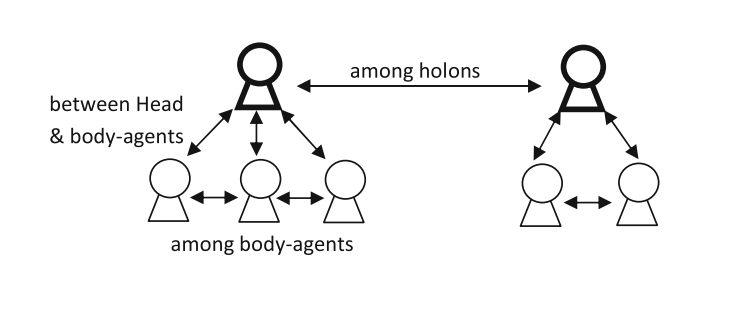
\includegraphics[width=0.7\linewidth]{img/holon_example}
	\caption{An example of the different negotiation between holons from \citet{beheshti2016negotiations}.}
	\label{fig:holonexample}
\end{figure}


\begin{figure}[h]
	
	\centering
	\begin{tikzpicture}
	
	\node[circle,draw,  minimum size=1cm] (A1) at  (0,0) {A$_1$};
	\node[circle,draw,  minimum size=1cm] (A2) at  (0,-1.5) {A$_2$};
	\node[circle,draw,  minimum size=1cm] (A3) at  (0,-3) {A$_3$};
	\node[circle,draw,  minimum size=1cm] (A4) at  (0,-4.5) {A$_4$};
	\node[circle,draw,  minimum size=1cm] (A5) at  (0,-6) {A$_5$};
	\node[circle,draw,  minimum size=1cm] (A6) at  (0,-7.5) {A$_6$};
	%\draw  (0,-2.5) ellipse (1 and 3.4);
	
	\node[ellipse,  draw, minimum height =9cm, minimum width = 2.5cm ] (A) at (0,-3.75) {Anion};
	
	\end{tikzpicture}
	\caption{Anion head and sub-agents}
	\label{fig:anion-head-sub}
	
\end{figure}

The following facts and rules would than be part of the Anion, meaning that a beginning towards an BDI in the agent can be made.

\begin{enumerate}
	\item
	Knowledge of anion head about the sub-agents:
	\begin{itemize}
		\item {$\{A_1, ..., A_6\}$ can process $a$ amount of water}
		\item {$\{A_1, ..., A_6\}$ needs to be cleaned after $b$ water}
		\item {$\{A_1, ..., A_6\}$ has filtered $c$ amount of water}
		\item {$\{A_1, ..., A_6\}$ needs $d$ base to clean}
		\item {$\{A_1, ..., A_6\}$ needs $e$ time to clean}
	\end{itemize}
	\item
	Currently $x$ amount of water being filtered 
	\item
	Currently $Z \subseteq \{A_1, ..., A_6\}$ filter being used for water filtering
	\item
	Currently $Y \subseteq \{A_1, ..., A_6\}$ filter being used for cleaning
	\item
	Currently $w$ amount of base being used for cleaning
\end{enumerate}

The use of these holons could allow an agent to reason about the environment, and act upon it accordingly.

\subsection{Utility function}
The requirement of a convex function forced the use of a specific, and highly theoretical function. This could be perfected using more expert input. Although an attempt was made, using a variable in the Mixbed ratio, this of course still is a highly theoretical and unrealistic representation.
\subsubsection{Reservation curve}
We have used a linear reservation curve for simplicity, since this eliminated the minimization (mixed integer programming) that would have been necessary if a truly curved function was used. An example is shown in \Cref{fig:anionreservationfunction}.
\begin{figure}[h]
	\centering
	\begin{tikzpicture}[domain=0.15:4]
	%\draw[very thin,color=gray] (0.01,0.01) grid (3.9,3.9);
	\draw[->] (0.02,0) -- (4.2,0) node[below] {$Water$};
	\draw[->] (0,0.02) -- (0,4.2) node[left] {$Base$};% node[pos=0.25, left] {$200 m^3 / hr$};
	\draw[color=black] plot (\x,{0.07*exp(\x)}) node[left] {$R_A$};
	\end{tikzpicture}
	\label{fig:anionreservationfunction}
	\caption{The reservation function for the Anion filter: the more water is filtered and given, the more base it requires.}
\end{figure}
\clearpage
\subsection{Continue negotiation after group agreement}
After the group has an agreement, the agents now allocate the resource as predefined (see \Cref{sec:design:mean}). This could be optimized to bilateral negotiation between the agents. Take the Mixbed and Anion for example: so if the group agrees to an allocation of 0.5 base, the Mixbed and anion can further negotiate how much of this 0.5 should be allocated to whom. This new bilateral negotiation is simpler, and due to the fact that it only contains a single issues, allows for quick determination.

\subsection{Extra concession strategies}
The many concession strategies, as shown in \Cref{sec:concessionstrat} allow for many strategies to be used. Further research could include using fraction, which was suggested as a good solution by \citet{wu2009efficient}. 
\subsection{Heuristic learning methods}
As shown in \Cref{sec:lit:learn}, heuristic learning methods can also be used to learn the desired utility function. This has not been done since the requirement of a convex utility functions forced the usage of predefined functions.

\todos